\usetikzlibrary{arrows.meta,positioning,shapes.geometric,calc}

\tikzset{
  >=Latex,
  flow/.style={
    font=\small,
    node distance=8mm and 9mm,
    line/.style={-Latex, semithick},
    block/.style={
      rectangle, draw, rounded corners,
      align=center,
      minimum width=2.0cm,
      inner sep=5pt,
      minimum height=6mm
    },
    decision/.style={
      diamond, draw,
      aspect=2.0,
      align=center,
      text width=1.8cm,
      inner sep=1pt
    },
    merge/.style={
      circle, draw,
      inner sep=0.8pt,
      minimum size=3.8mm
    }
  }
}

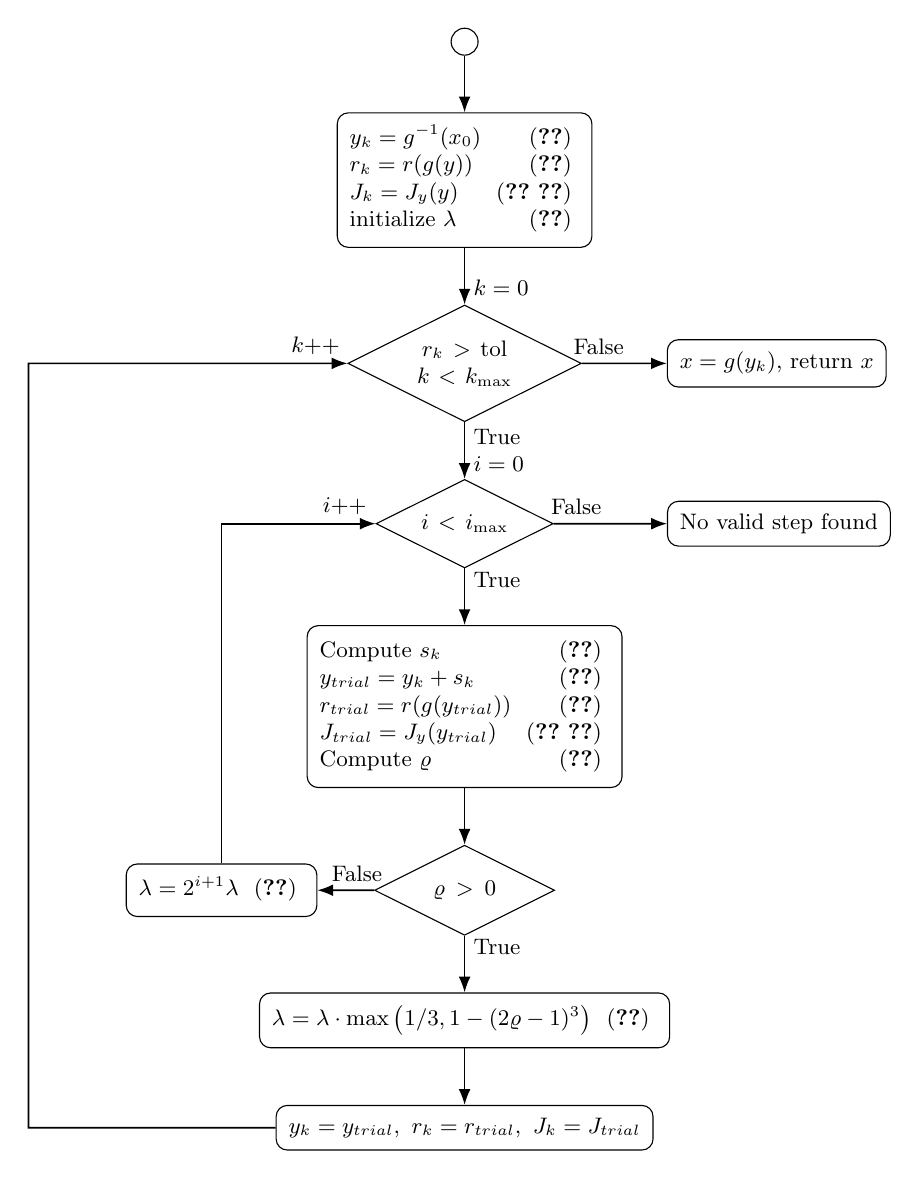
\begin{tikzpicture}[flow, scale=0.90, transform shape]
{ %% scope guard
\setlength{\tabcolsep}{3pt}
% ---- First part
\node[merge] (start) {};
\node[block, below=of start] (b0) {
\begin{tabular}{@{}lr@{}}
    $y_k = g^{-1}(x_0)$ & (\ref*{eq:g_func})\\
    $r_k = r(g(y))$ & (\ref*{eq:residual})\\
    $J_k = J_y(y)$ & (\ref*{eq:jacobian} \ref*{eq:Jy}) \\
    initialize $\lambda$ & (\ref*{eq:init_lambda}) \\
\end{tabular}
};

\draw[line] (start) -- (b0);

% Main loop
\node[decision, below=of b0] (d1)
{$\lVert r_k\rVert > \mathrm{tol}$ \\ $k < k_{\max}$};
\draw[line] (b0) -- node[right,pos=0.7]{$k=0$} (d1);

% Return x
\node[block, right=12mm of d1] (ret) {$x=g(y_k)$,\ return $x$};
\draw[line] (d1.east) -- node[above,pos=0.2]{False} (ret.west);

% Continue False
%\node[block, below=of d1] (d2) {$i=0$};

% Inner damping loop
\node[decision, below=of d1] (d2) {$i<i_{\max}$};
\draw[line] (d1.south) -- node[right,pos=0.5,align=left]{True\\$i=0$} (d2);


% Max iter reached
\node[block, right=16mm of d2] (retF) {No valid step found};
\draw[line] (d2.east) -- node[above,pos=0.2]{False} (retF.west);

% Inner loop body
\node[block, below=of d2] (inner_compute){
\begin{tabular}{@{}lr@{}}
    Compute $s_k$ & (\ref*{eq:sk_lm_solve})\\
    $y_{\text{trial}}=y_k+s_k$ & (\ref*{eq:step_update_rule})\\
    $r_{\text{trial}}=r(g(y_{\text{trial}}))$ & (\ref*{eq:residual})\\
    $J_{\text{trial}}=J_y(y_{\text{trial}})$ & (\ref*{eq:jacobian} \ref*{eq:Jy})\\
    Compute $\varrho$ & (\ref*{eq:gain_ratio_solve})
\end{tabular}
};
\draw[line] (d2) -- node[right,pos=0.2]{True} (inner_compute);

% End inner loop?
\node[decision, below=of inner_compute] (d3) {$\varrho>0$};
\draw[line] (inner_compute) -- (d3);

% False, loop back inner loop
\node[block, left=8mm of d3] (upd)
{
\begin{tabular}{@{}lr@{}}
$\lambda=2^{i+1} \lambda$ & (\ref*{eq:inc_lambda})
\end{tabular}
};
\draw[line] (d3.west) -- node[above,pos=0.3]{False} (upd.east);
\draw[line] (upd.north) |-  node[above,pos=0.9]{$i{+}{+}$} (d2.west);

% True, continue
\node[block, below=of d3] (lambda_update) {
\begin{tabular}{@{}lr@{}}
$\lambda = \lambda \cdot \max \left( 1/3, 1-(2\varrho-1)^3 \right)$ & (\ref*{eq:dec_lambda})
\end{tabular}
};
\draw[line] (d3.south) -- node[right,pos=0.2]{True} (lambda_update.north);



\node[block, below=of lambda_update] (update_k_iter) {
$y_k = y_{\text{trial}},\ r_k=r_{\text{trial}},\ J_k=J_{\text{trial}}$};
\draw[line] (lambda_update) -- (update_k_iter);



% Loop back
\coordinate (loopcol) at ($(d1.west)+(-45mm,0)$);
\coordinate (back1) at (loopcol |- update_k_iter.west);
\coordinate (back2) at (loopcol |- d1.west);
\draw[line] (update_k_iter.west) -- (back1) -- (back2) -- node[above,pos=0.9]{$k{+}{+}$} (d1.west);

} %% scope guard
\end{tikzpicture}



% old lambda update
% % True, update varrho
% \node[decision, below=of d3] (d4) {$\varrho>0.75$};
% \draw[line] (d3.south) -- node[right,pos=0.4]{True} (d4.north);
% % varrho>0.75 == True
% \node[block, below=of d4] (lamdec)
% {$\lambda=\max(\lambda/3,\ \lambda_{\min})$};
% \draw[line] (d4) -- node[right]{True} (lamdec);

% % varrho>0.75 == False
% \node[decision, right=10mm of d4] (d5) {$\varrho<0.25$};
% \draw[line] (d4.east) -- node[above]{False} (d5.west);

% % varrho<0.25 == True
% \node[block, below=of d5] (laminc) {$\lambda=2\lambda$};
% \draw[line] (d5) -- node[right]{True} (laminc);

% % merge all
% \node[below=2mm of lamdec] (mp) {};
% \node[block, below=of mp] (update_k_iter) {$\nu=2\nu,\ y_k = y_{\text{trial}},\ r_k=r_{\text{trial}},\ J_k=J_{\text{trial}},\ k{+}{+}$};
% \draw[line] (mp) -- (update_k_iter);
% \draw[line] (lamdec.south) -- (update_k_iter.north);
% \draw[line] (laminc.south) |- (mp.center) -- (update_k_iter.north);
% \draw[line] (d5.east) -- ++(6mm,0) node[above]{False} -- ++(6mm,0) |- (mp.center) -- (update_k_iter.north);